\documentclass[sigconf]{acmart}

\usepackage{booktabs}    % For formal tables
\usepackage{mathtools}
\usepackage{setspace}
\usepackage{subcaption}


% For subcaption
\captionsetup[subfigure]{labelformat=simple}
\renewcommand{\thesubfigure}{(\alph{subfigure})}


% Copyright
%\setcopyright{none}
%\setcopyright{acmcopyright}
%\setcopyright{acmlicensed}
\setcopyright{rightsretained}
%\setcopyright{usgov}
%\setcopyright{usgovmixed}
%\setcopyright{cagov}
%\setcopyright{cagovmixed}


% DOI
\acmDOI{10.1145/nnnnnnn.nnnnnnn}


% ISBN
\acmISBN{978-x-xxxx-xxxx-x/YY/MM}


% Conference
\acmConference[GECCO '19]{the Genetic and Evolutionary Computation Conference 2019}{July 13--17, 2019}{Prague, Czech Republic}
\acmYear{2019}
\copyrightyear{2019}


%\acmArticle{4}
\acmPrice{15.00}


% These commands are optional
%\acmBooktitle{Transactions of the ACM Woodstock conference}
%\editor{Jennifer B. Sartor}
%\editor{Theo D'Hondt}
%\editor{Wolfgang De Meuter}


\begin{document}
\title{Stabilized Training of Generative Adversarial Networks by a Genetic Algorithm}


%% Authors
\author{Hwi-Yeon Cho}
\orcid{0000-0002-4604-2578}
\affiliation{%
  \institution{Department of Computer Science, Kwangwoon University}
  \city{Seoul}
  \country{Republic of Korea}
}
\email{hwyn.cho@gmail.com}

\author{Yong-Hyuk Kim}
\orcid{0000-0002-0492-0889}
\affiliation{%
  \institution{Department of Computer Science, Kwangwoon University}
  \city{Seoul}
  \state{Republic of Korea} 
}
\email{yhdfly@kw.ac.kr}

% The default list of authors is too long for headers.
\renewcommand{\shortauthors}{H.-Y. Cho et al.}


\begin{abstract}
Generative adversarial networks (GAN) facilitate the learning of probability distributions of complex data in the real world, and allow neural networks to generate the distribution. GANs (GAN and its variants) exhibit excellent performance in applications like image generation and video generation. However, GANs sometimes experience problems during training with regard to the distribution of real data. We applied a genetic algorithm to improve and optimize the GAN’s training performance. As a result, the convergence speed and stability during the training process improved compared to the conventional GAN.
\end{abstract}


%
% The code below should be generated by the tool at http://dl.acm.org/ccs.cfm
% Please copy and paste the code instead of the example below. 
%
\begin{CCSXML}
<ccs2012>
  <concept>
    <concept_id>10010147.10010257.10010293.10011809.10011812</concept_id>
    <concept_desc>Computing methodologies~Genetic algorithms</concept_desc>
    <concept_significance>500</concept_significance>
  </concept>

  <concept>
    <concept_id>10010147.10010257.10010293.10010294</concept_id>
    <concept_desc>Computing methodologies~Neural networks</concept_desc>
    <concept_significance>300</concept_significance>
  </concept>
</ccs2012>
\end{CCSXML}


\ccsdesc[500]{Computing methodologies~Genetic algorithms}
\ccsdesc[300]{Computing methodologies~Neural networks}


\keywords{genetic algorithm, neural networks}

\maketitle


% Section 1
\section{Introduction}
\label{sec:introduction}
Generative adversarial networks (GAN)~\cite{DBLP:conf/nips/GoodfellowPMXWOCB14} constitute one of the major methods used for learning and generating complex data in the real world. To generate meaningful data that are similar to real data, GANs (GAN and its variants) adversarially train not only the generator but also the discriminator to classify real samples and generated fake samples. In recent years, such GANs have been successfully applied to applications like image generation and editing.\\
However, when the distribution of the training dataset and the distribution of the generated samples are not similar, the GAN experiences issues with training. To solve this, deep convolutional GAN (DCGAN)~\cite{DBLP:journals/corr/RadfordMC15} was developed to apply a convolutional structure to a conventional GAN that uses multilayer perceptron. Moreover, evolutionary GAN~\cite{DBLP:journals/corr/abs-1803-00657} was developed to apply evolutionary computation to the adversarial training. Specifically, generators generate offspring through mutation, and the population of generators evolves while preserving only the good generators.\\
We sought to improve and optimize the GAN’s training performance by applying a GA. In particular, this was achieved by focusing on the oscillation phenomenon, in which the training is unstable and model does not converge even if trained for a significant amount of time. This study aims to improve the discrimination performance of the discriminator using the GA and to improve the generation performance of the generator. Experiments were conducted by applying the proposed method to the actual MNIST dataset. The results yielded performance improvements during the training process compared to the conventional GAN.


% Section 2
\section{Generative Adversarial Networks Combined with a Genetic Algorithm}
\subsection{GAN}
\label{sec:gan}
The GAN learns the minimax game between the generative network \(G\) and the discriminative network \(D\). The \(G\) receives the latent vector \(z \sim p\left(z\right)\) (sampled from a normal distribution) as input, and outputs new data \(G\left(z\right) \sim p_{g}\) that approaches the data distribution \(p_{data}\). On the other hand, the \(D\) discriminates the real data \(x \sim p\left(x\right)\) and the data \(G\left(z\right) \sim p_{g}\left(G\left(z\right)\right)\) generated by \(G\). Such a training process for the GAN can be expressed by the following equation.
\begin{equation}
    \min\limits_{G} \max\limits_{D} \mathbb{E}_{x \sim p\left(x\right)}\left[\log D\left(x\right)\right] + \mathbb{E}_{z \sim p\left(z\right)}\left[\log \left(1 - D\left(G\left(z\right)\right)\right)\right]
\end{equation}
If the training is continued in this manner, then, at the end, \(p_{data} = p_{g}\), which represents the state in which the \(D\) cannot discriminate between the real and the fake, i.e., \(D\left(x\right) = D\left(G\left(z\right)\right) = \frac{1}{2}\).

\subsection{Parameters of GA}
\label{sec:ga-parameters}
A population of the same size as the GAN’s training batch size was chosen, and each chromosome was a fake sample (i.e., \(G\left(z\right)\)) generated by the \(G\). The fitness of the chromosome was the \(D\)'s discrimination value (i.e., \(D\left(G\left(z\right)\right)\)). Roulette wheel selection was used for the selection type, and arithmetic recombination crossover for the crossover type. The mutation was carried out by adding an arbitrary number between \(-0.05\) and \(+0.05\) to each gene with a probability of \(10\%\). When the fitness of the offspring was higher than that of the individual with the lowest fitness of the conventional population, the worst individual was replaced by the offspring.

\subsection{GAN combined with GA}
\label{sec:ga-gan}
A conventional GAN trains the \(D\) and \(G\) alternately, as shown in Figure~\ref{fig:1-a}. Because of this, at a certain step, a problem may occur whereby the training of the \(D\) and the training of the \(G\) cancel each other out. By applying the GA to each training step, as shown in Figure~\ref{fig:1-b}, we attempted to improve the discrimination ability of the \(D\) and, accordingly, improve the performance of the \(G\).\\
First, the initial population was populated with the fake samples (i.e., chromosome) generated by the \(G\), and the fitness of each fake sample was calculated. The samples of high fitness (samples that were discriminated as real by the \(D\)) were selected, and the population was evolved by using the parameters introduced in Section~\ref{sec:ga-parameters}. By supplying it with fake samples from the evolved population (i.e., \(G'(z)\)), the \(D\) was trained. Through this process, the \(D\) should be perform better, in turn causing the \(G\) to improve even more.

\begin{figure}[h!]
\centering
\subcaptionbox{
    Conventional GAN
    \label{fig:1-a}
}{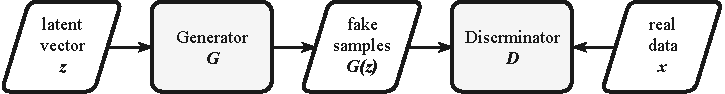
\includegraphics[width=\columnwidth]{figure-1-a}}\\
\subcaptionbox{
    GAN combined with GA
    \label{fig:1-b}
}{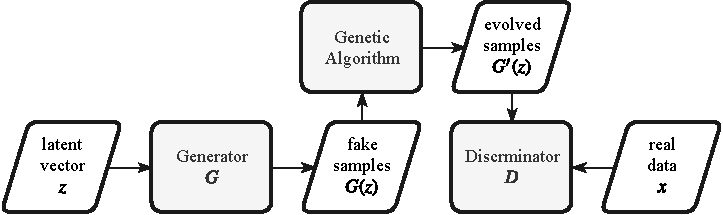
\includegraphics[width=\columnwidth]{figure-1-b}}
\caption{Conventional GAN and the proposed GAN}
\label{fig:1}
\end{figure}


% Section 3
\section{Results and Analysis}
\label{sec:results}
In this section, the experiments and analysis are discussed for tasks of several generations to evaluate the proposed GAN combined with GA. The data used in the experiments were from the MNIST dataset (a dataset that consists of handwritten digits between \(0\) and \(9\)), which are widely used for training and validation in machine learning. We trained the GAN and performed the data generation experiment by separating the data by each digit. The performance was measured using the loss (binary cross-entropy) of the discriminator and the generator before and after the application of the GA to the conventional GAN. The binary cross-entropy is calculated from the equation below. When the GAN is trained and \(D\left(x\right)=D\left(G\left(z\right)\right) = \frac{1}{2}\) is obtained, the loss value becomes \(0.69\), at which point model has converged.
\begin{equation}
    H\left[X\right] = -\left[P\left(X=0\right)\log{P\left(X=0\right) + P\left(X=1\right)\log{P\left(X=1\right)}}\right]
\end{equation}
Figure~\ref{fig:2} compares the loss of the discriminator and the generator before and after application of the GA to the GAN. Although these did not converge before or after application of the GA to the GAN, the training proceeded more stably and more convergently when the GA was applied. Figure~\ref{fig:3} shows the kernel density estimate plot for the distribution of digit \(0\) and the distribution of samples generated during the training of the GAN. For each step, the data generated by the GAN combined with GA closely matched the distribution of the actual data, and the training and generation performance improved slightly. Because of the space limit of this paper, we did not include all results. As representatives, we compared the results of digit \(0\) and step \(420\).

\begin{figure}[t]
\centering
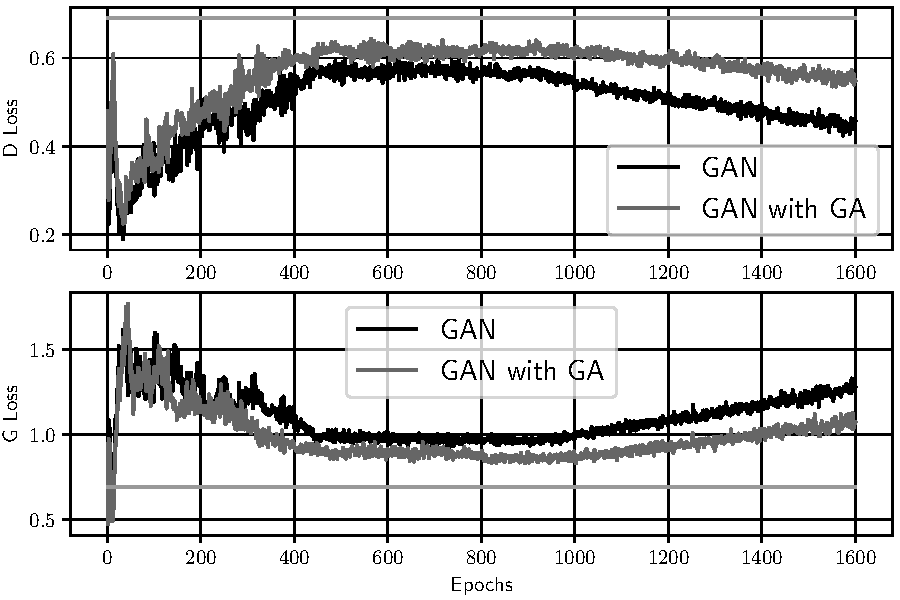
\includegraphics[width=\columnwidth]{figure-2}
\caption{Comparison of loss for each step of GAN during training for the digit \(0\)}
\label{fig:2}
\end{figure}

\begin{figure}[t]
\centering
\subcaptionbox{
    Conventional GAN
    \label{fig:3-a}
}{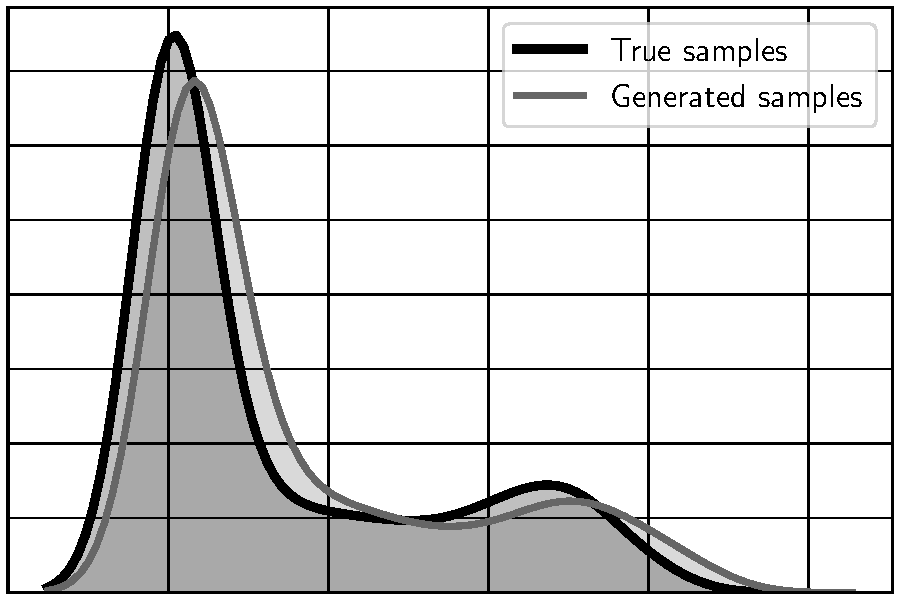
\includegraphics[width=0.46\columnwidth]{figure-3-a}}
\subcaptionbox{
    GAN combined with GA
    \label{fig:3-b}
}{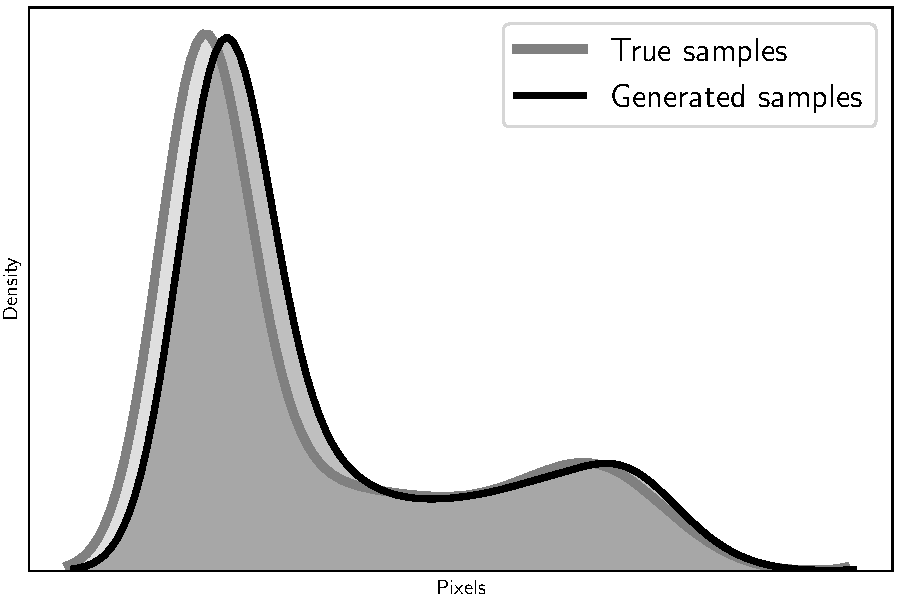
\includegraphics[width=0.46\columnwidth]{figure-3-b}}
\caption{Comparison of generation performance with GA at step 420}
\label{fig:3}
\end{figure}


% Section 4
\section{Conclusion}
\label{sec:conclusion}
GANs constitute one of the major methods used in data generation and editing. Additionally, the GA approach is widely used in various optimization problems. This study proposed an approach in which a GA was utilized to address the GAN’s issues and improve performance. When the GA was used, the generated samples evolved in a diverse manner and the discriminator was able to discriminate more stably. Although there was no noticeably large improvement, it was confirmed that it is possible to solve some of the issues present in GANs and improve performance by applying a GA. In the future, we plan to conduct a more in-depth study on methods for improving GANs by applying a GA and improving the generation performance.



\begin{acks}
\footnotesize
This research was supported by a grant [KCG-01-2017-05] through the Disaster and Safety Management Institute funded by Korea Coast Guard of Korean government.
\par
\end{acks}


\bibliographystyle{ieeetr}
\bibliography{bibliography}


\end{document}
